\clearpage
\section{Multiple Output Converter}
Another advantage of combining a SCC with inductors is to enable multiple output voltages with a single power stage. \citeauthor{2012Kumar}~\cite{2012Kumar} presented a Triple Output Fixed Ratio Converter (TOFRC) where a 2:1 Ladder converter is combined with two inductors in order to provide three fixed output voltages with a single SCC stage.

\subsection{The Output Trans-Resistance Model}

When considering a converter with multiple outputs, the load effects have to be taken into account for all the outputs. Actually, when the converter is loaded, it produces a voltage drop throughout outputs of the converter. Therefore, the output current of one output node has an influence to the other outputs. In order to model these effects a new model based on trans-resistance parameters is proposed.

\begin{figure}[!h]
\centering
\ctikzset { bipoles/length=1cm}
\begin{circuitikz}[american voltages, scale=0.65]
\draw
    (0,0) to[V = $ m_1  v_{src}  $] (0,3)
    (3,3) to[american controlled voltage source,l_=$i_1 z_{11} + i_2 z_{12} + \cdots + i_n z_{1n} $] (0,3)
    (3,3) to[short,i>_=$i_1$,-o] (4,3)
    (4,0) to[short,o-] (0,0)
    (4,3) to[open,v^=$v_1$] (4,0);

\draw
    (8,0) to[V = $ m_n  v_{src}  $] (8,3)
    (11,3) to[american controlled voltage source,l_=$i_1 z_{n1} + i_2 z_{n2} + \cdots + i_n z_{nn} $] (8,3)
    (11,3) to[short,i>_=$i_n$,-o] (12,3)
    (12,0) to[short,o-] (8,0)
    (12,3) to[open,v^=$v_n$] (12,0);

\end{circuitikz}
\caption{Output trans-resistance model of a switched capacitor converter.}
\label{fig:scc_model_tr}
\end{figure}

The proposed model is shown in Figure\ref{fig:scc_model_tr}; as it can be seen, each output is represented using two controlled voltage sources connected in anti-series. One source provides the \emph{target voltage}  associated with the output, taking the value from the input voltage, $v_{src}$, multiplied by the respective conversion ratio associated to that output, $m_x$.

The other source, produces a voltage droop associated with the losses in the converter. The current delivered by each loaded node adds a specific contribution to the converter losses. Therefore, this voltage source takes the value given by the linear combination of all the converter output currents weighted by their associated trans-resistance factor $z$.

The trans-resistance factor $z_{xy}$ produces a voltage drop at the output $x$ proportional to the charge (\emph{i.e}. current) delivered by the output $y$.  It can be seen that the trans-resistance factor $z_{xx}$ corresponds to the voltage drop of the same output where the current is delivered, thus this parameter is  the output impedance for that node. Since all the trans-resistance factors relate current to voltage, they have are expressed in \emph{Ohms}.

With the proposed model, the converter behavior can be obtained as
\begin{equation}
 \mathbf{v_o} = -\mathbf{Z} \cdot \mathbf{i_o} + \mathbf{m} \cdot v_{src},
 \label{eq:admit_sol}
\end{equation}
where $\mathbf{Z}$ is the \emph{trans-resistance matrix}, which is symmetric in two phase converters.


\subsection{Model duality: Power losses and Trans-resistance model}
\begin{figure}[!h]
\centering
\ctikzset { bipoles/length=1cm}
\begin{circuitikz}[american voltages, scale=0.65]
\draw
    (0,0) to[V = $ m_1  v_{src}  $] (0,3)
    (3,3) to[american controlled voltage source,l_=$i_1 z_{11} + i_2 z_{12} $] (0,3)
    (3,3) to[short,i>_=$i_1$,-o] (4,3)
    (4,0) to[short,o-] (0,0)
    (4,3) to[open,v^=$v_1$] (4,0);

\draw
    (8,0) to[V = $ m_2  v_{src}  $] (8,3)
    (11,3) to[american controlled voltage source,l_=$i_1 z_{21} + i_2 z_{22} $] (8,3)
    (11,3) to[short,i>_=$i_2$,-o] (12,3)
    (12,0) to[short,o-] (8,0)
    (12,3) to[open,v^=$v_2$] (12,0);

\end{circuitikz}
\caption{Two output converter.}
\label{fig:model_duality}
\end{figure}
Using the trans-resistance matrix $\mathbf{Z}$ the losses of the converter can be computed. For a two output converter, modeled as shown in Figure~\ref{fig:model_duality}, the losses associated to each output would be
\begin{equation}
 P_{o1} = i_1^2 ~ z_{11} + i_1 ~ i_2 ~ z_{12}
 \label{eq:ploss_1}
\end{equation}

\begin{equation}
 P_{o2} = i_1 ~ i_2 z_{21} + i_2^2 ~ z_{22},
 \label{eq:ploss_2}
\end{equation}
and the total converter losses are
\begin{equation}
 P_{total} = i_1^2 ~ z_{11} + i_2^2 ~ z_{22} +  i_1 ~ i_2 ~ z_{12} ~ z_{21}  .
 \label{eq:ploss_3}
\end{equation}
%\subsubsection{Slow Switching Limit}
Using the the charge flow analysis  described in the previous section, the total losses of a two output converter can be computed as well. In order to make the analysis less cumbersome, the phases are eluded and losses are computed in a single capacitor for the SSL. The results can be extended for any converter with any number of phases and capacitors.

In the case of a multiple-output converter, each of the individual outputs produces a \emph{redistributed} flow of charge through the capacitors that can be individually quantified, being $g_{i,1}$ associated to the first output, $g_{i,2}$ associated to the second output, etc. The total \emph{redistributed} charge is the sum of each individual contributions as
\begin{equation}
 g_i =  (g_{i,1} ~ q_{o,1} +  g_{i,2} ~ q_{o,2}).
 \label{eq:g_i_total}
\end{equation}
Substituting~\eqref{eq:g_i_total} in~\eqref{eq:pwr_ssl} the losses produced in capacitor $c_i$ of the two output converter are
\begin{equation}
 P_{c_{i}} = f_{sw} \frac{1}{2 ~ c_i} (g_{i,1} ~ q_{o,1} +  g_{i,2} ~ q_{o,2})^2.
 \label{eq:ploss_c_2}
\end{equation}
expanding terms and substituting $q_{o,1}=i_1/f_{sw}$ and $q_{o,2}=i_2/f_{sw}$ into~\eqref{eq:ploss_c_2}  yelds
\begin{equation}
 P_{c_{i}} =  \frac{1}{2 ~ f_{sw} ~ c_i} (i_1^2 ~g_{i,1}^2  +  i_2^2 ~ g_{i,2}^2 + 2 ~ i_{1} ~ i_{2} ~ g_{i,1}~g_{i,2} ).
 \label{eq:ploss_c_3}
\end{equation}
It can be seen that the trans-resistance parameters of~\eqref{eq:ploss_3} can be directly matched with the \emph{redistributed charge flow multipliers} in ~\eqref{eq:ploss_c_3} as
\begin{center}
    \renewcommand{\arraystretch}{2}
    \begin{tabular} {l c c c }
	$z_{11}$ & = & $\raisebox{0.8ex}{$g_{i,1}^2$}\big/ \raisebox{-0.6ex}{$2 f_{sw} c_i$}$ & $[\Omega] $\\
	$z_{22}$ & = & $\raisebox{0.8ex}{$g_{i,2}^2$}\big/ \raisebox{-0.6ex}{$2 f_{sw} c_i$} $& $[\Omega]$\\
	$z_{12} + z_{21} $ & = & $\raisebox{0.8ex}{$g_{i,1}g_{i,2}$}\big/ \raisebox{-0.6ex}{$ f_{sw} c_i$} $& $ [\Omega]$
    \end{tabular}
\end{center}
Therefore the general expression of a trans-resistance parameter for the
SSL is obtained using the \emph{redistributed charge multipliers} as
\begin{equation}
  z_{ssl,xx} =  \frac{1}{2 f_{sw}} \sum_{i=1}^{caps.} \sum_{j=1}^{phas.}
  \frac{ \left ( g_{i,x}^j \right )^2 } {c_i}.
 \label{eq:z_ssl_xx}
\end{equation}

\begin{equation}
  z_{ssl,xy} + z_{ssl,yx} =  \frac{1}{f_{sw}} \sum_{i=1}^{caps.} \sum_{j=1}^{phas.}
  \frac{g_{i,x}^j g_{i,y}^j}{c_i}.
 \label{eq:z_ssl_xy}
\end{equation}
%\subsubsection{Fast Switching Limit}
The same analysis can be done for the FSL, but in this case the losses are compute for a single resistor.
As in the SSL case of a multiple-output converter, each of the individual outputs produces a charge flow through the switches that can be individually quantified, being $ar_{i,1}$ associated to the first output, $ar_{i,2}$ associated to the second output, etc. The total \emph{switch} charge multiplier is the sum of each individual \emph{switch} multiplier as
\begin{equation}
 ar_i =  (ar_{i,1} ~ q_{o,1} +  ar_{i,2} ~ q_{o,2}).
 \label{eq:ar_i_total}
\end{equation}
Substituting~\eqref{eq:ar_i_total} in~\eqref{eq:pwr_ssl}, the power dissipated in $r_i$ of the two output converter are
\begin{equation}
 P_{r_{i}} =  \frac{r_i}{D} (i_1^2 ~ar_{i,1}^2  +  i_2^2 ~ ar_{i,2}^2 + 2 ~ i_{1} ~ i_{2} ~ ar_{i,1}~ar_{i,2}),
 \label{eq:ploss_r_1}
\end{equation}
leading to a similar polynomial solution of the previous case. Hence the general expression for FSL is
\begin{equation}
  z_{fsl,xx} =   \sum_{i=1}^{swts.} \sum_{j=1}^{phas.}
  \frac{r_{i}}{D^j} \left ( ar_{i,x}^j \right )^2,
 \label{eq:z_fsl_xx}
\end{equation}
\begin{equation}
  z_{fsl,xy} + z_{fsl,yx} =   \sum_{i=1}^{swts.} \sum_{j=1}^{phas.}
  \frac{r_{i}}{D^j} ar_{i,x}^j ar_{i,y}^j,
 \label{eq:z_fsl_xy}
\end{equation}

It can be seen from~\eqref{eq:z_ssl_xy} and ~\eqref{eq:z_fsl_xy} that there are not individual solutions for the cross trans-resistance elements $z_{xy}$ and $z_{yx}$. Actually the individual value of these parameters is related to the order of sequence of the converter's circuit modes. In the case of a two-phase converters, the parameters are equal, thus $Z_{xy} = z_{yx}$,  which transforms $\mathbf{Z}$ matrix to a symmetric matrix. At the same time it reduces the generic expression to two:
\begin{equation}
  z_{ssl,xy}  =  \frac{1}{2~f_{sw}} \sum_{i=1}^{caps.} \sum_{j=1}^{phas.}
  \frac{g_{i,x}^j g_{i,y}^j}{c_i}.
 \label{eq:z_ssl_xy_2ph}
\end{equation}
\begin{equation}
  z_{fsl,xy} =   \sum_{i=1}^{swts.} \sum_{j=1}^{phas.}
  \frac{r_{i}}{D^j} ar_{i,x}^j ar_{i,y}^j,
 \label{eq:z_fsl_xy_2ph}
\end{equation}

For multiple-phase converters, the relation between the sequentiality of the circuit modes and the cross trans-conductance has not be yet found. Nevertheless multiple-phase converters are beyond the scope of this dissertation, since they have not been used for the H-SCCs of this work.

\subsection{Trans-resistance Parameters Methodology}

Based on the \emph{charge flow analysis} for current-loaded SCCs, each converter output has three associated sets of charge flow vectors per switching phase. Thus, for a given converter, the different vector types can be collected in a matrix, where each column corresponds to a converter output and each row corresponds to a circuit component.

Therefore the \emph{charge flow multipliers} are collected in a matrix as
\begin{equation}
 \mathbf{A}^j =
   \bordermatrix { ~ & out_1 & out_2 & ~ & out_n \cr
     v_{in} & a_{1,1}^j  & a_{1,2}^j & \cdots & a_{1,n}^j \cr
     C_1    & a_{2,1}^j  & a_{2,2}^j & \cdots & a_{2,n}^j \cr
      ~     & \vdots     & \vdots & \ddots & \vdots \cr
     C_p    & a_{p,1}^j  & a_{p,2}^j & \cdots & a_{p,n}^j \cr},
 \label{eq:A_matrix}
\end{equation}
where the elements of the first row  $a_{1,x}^j$ corresponds to the \emph{charge flow multiplier}  delivered by the input voltage source associated to the charge flow through the $x$\emph{-th} output. The remaining elements after the first row are associated with the charge flow in the capacitors. Therefore $a_{1,1}$ is the net charge flow in capacitor $C_1$ due to the charge delivered at the $1st$ output node of a converter with $p$ capacitors and $n$ outputs.

Likewise, the \emph{charge pumped multipliers} are collected in the following matrix
\begin{equation}
 \mathbf{B}^j =
   \bordermatrix { ~ & out_1 & out_2 & ~ & out_n \cr
     C_1  & b_{1,1}^j  & b_{1,2}^j & \cdots & b_{1,n}^j \cr
     C_2  & b_{2,1}^j  & b_{2,2}^j & \cdots & b_{2,n}^j \cr
      ~   & \vdots     & \vdots & \ddots & \vdots \cr
     C_p  & b_{p,1}^j  & b_{p,2}^j & \cdots & b_{p,n}^j \cr}
 \label{eq:A_matrix},
\end{equation}
where all the elements are associated with the converter capacitors.

On the other hand, the \emph{switch charge flow multipliers} lead to the following matrix
\begin{equation}
 \mathbf{Ar}^j =
   \bordermatrix { ~ & out_1 & out_2 & ~ & out_n \cr
     sw_1  & ar_{1,1}^j  & ar_{1,2}^j & \cdots & ar_{1,n}^j \cr
     sw_2  & ar_{2,1}^j  & ar_{2,2}^j & \cdots & ar_{2,n}^j \cr
      ~    & \vdots     & \vdots & \ddots & \vdots \cr
     sw_p  & ar_{p,1}^j  & ar_{p,2}^j & \cdots & ar_{p,n}^j \cr}.
 \label{eq:A_matrix}
\end{equation}
where all the elements are associated with the converter switches. This matrix can be extended with the Equivalent Series Resistance (ESR) of the capacitors, but for the sake of clarity they are not included in the present calculations yet.

 The converter is described with two trans-resistance matrix: one for the SSL, $\mathbf{Z_{ssl}}$, and another for the FSL, $\mathbf{Z_{fsl}}$.

\subsubsection{Slow Switching Limit Trans-resistance Matrix}

The \emph{redistributed} charge flow multipliers matrix can be obtained from the
matrices $\mathbf{A}$ and $\mathbf{B}$  as
\begin{equation}
 \mathbf{G}^j = \mathbf{A}_{(2:end,1:end)}^j - D^j \mathbf{B}^j,
 \label{eq:R_matrix}.
\end{equation}
The \emph{redistributed charge} corresponds to the charge that flows between capacitors; therefore it is the root cause of
losses associated with the SSL operation regime \cite{SeemanPhD06}.

The SSL trans-resistance factors can be individually obtained from the redistributed charge multipliers as described in \eqref{eq:z_ssl}. In order to obtain directly the trans-resistance matrix, the operation in \eqref{eq:z_ssl} is performed in  two steps. First, the outer product of  each row of $\mathbf{G}^j$ is taken with itself as
\begin{equation}
 \mathbf{K}_i^j =[\mathbf{G}_{(i,1:end)}^j ]^T \mathbf{G}_{(i,1:end)}^j ,
 \label{eq:K_matrix}
\end{equation}
where the matrix $\mathbf{K_i}$ contains all the possible products of the  $i^{th}$ row. Since each row in $\mathbf{G}$ is associated with a capacitor, there is a matrix $\mathbf{K_i}$ for each capacitor $C_i$.
Second, with the set of $\mathbf{K}$ matrices the trans-resistance matrix is obtained as
\begin{equation}
 \mathbf{Z_{ssl}} = \frac{1}{2 F_{sw}} \sum_{j=1}^{phas.} \sum_{i=1}^{caps.} \frac{1}{C_i} \mathbf{K}_i^j.
 \label{eq:G_ssl}
\end{equation}

\subsubsection{Fast Switching Limit trans-resistance Matrix}
For the FSL, the trans-resistance matrix is obtained using the switch charge multipliers
contained in matrix $\mathbf{Ar}$. The operation to obtain the trans-resistance matrix as described
in \eqref{eq:z_ssl_xy_2ph} is performed in two steps. First, a set of matrices are obtained by taking the outer product
of each row of $\mathbf{Ar}$ with itself as
\begin{equation}
 \mathbf{Kr}_i^j = \mathbf{Ar}_{(i,1:end)}^j [\mathbf{Ar}_{(i,1:end)}^j]^T,
 \label{eq:Kr_matrix}
\end{equation}
yielding a matrix for each row in $\mathbf{Ar}$ associated with a switch \emph{on}-resistance ($r_{i}$). Second, with the set of matrices $\mathbf{Kr}$ the FSL trans-resistance matrix is obtained as
\begin{equation}
 \mathbf{Z_{fsl}} =  \sum_{i=1}^{swts.} \sum_{j=1}^{phas.} \frac{_{i}}{D^j}
\mathbf{Kr}_i^j ,
 \label{eq:G_fsl}
\end{equation}

\subsubsection{Total Trans-resistance Matrix}
The total trans-resistance values are approximated using~\eqref{eq:r_scc} as
\begin{equation}
 \mathbf{Z}_{(x,y)} = \sqrt{\mathbf{Z_{ssl,(x,y)}}^2 + \mathbf{Z_{fsl,(x,y)}}^2}.
 \label{eq:G_total}
\end{equation}

\subsubsection{Conversion Ratio Vector }

The conversion ratio vector is obtained as
\begin{equation}
 \mathbf{m} = \sum_{j=1}^{phas.}[\mathbf{A}^j_{(1,1:end)}]^T.
 \label{eq:m_equation}
\end{equation}

\subsection{Experimental Model Validation}

The trans-impedance matrix is determined for the converter of Figure~\ref{fig:2_1_two_outs}. The results of the model parameters are compared with both  PLECS\footnote[1]{Behavioral circuit simulator running on Matlab \textsuperscript{\textregistered}-Simulink \textsuperscript{\textregistered}} simulations and experiments.

\begin{figure}[t]
\ctikzset { bipoles/length=1cm}
\centering
\begin{circuitikz}[american voltages,scale=0.6]
    \draw
            %Input Supply
            %(0,0)  to[V=$v_{src}$]
            %Draw Switches
            %(0,10)  --
            (5,10.4) node[anchor=south] {$v_{src}$}
            (5,10) node[rground, yscale=-1] {}
            to[switch=$s_1$] %S1
            (5,8)   to[switch=$s_2$] %S2
            (5,6)   to[switch=$s_3$] %S3
            (5,4)   to[switch=$s_4$]
            (5,2)   node[sground] {};


    \draw %Capacitor C1
           (5,4) -- (3,4)
           to[pC,l^=$c_1$]
           (3,8) -- (5,8);

    \draw %Capacitor C2
           (5,2) -|  (7,4)
           to[pC,l_=$c_2$] (7,6) --
           (5,6);

    \draw (5,8) -- (8,8) to[short,i=$i_3$,-o] (10,8) node[anchor=west] {$v_{3}$} ;
    \draw (5,6) -- (8,6) to[short,i=$i_2$,-o] (10,6) node[anchor=west] {$v_{2}$} ;
    \draw (5,4) -- ([hs]7,6 |- 5,4) arc(180:0:\radius) -- (8,4) to[short,i=$i_1$,-o] (10,4) node[anchor=west] {$v_{1}$} ;


     \end{circuitikz}
\caption{ Circuit used for the experimental setup, 2:1 SCC, presenting all the available outputs. In the experimental setup the outputs were loaded with constant current sinks. }
\label{fig:2_1_two_outs}
\end{figure}


The circuit is solved for matrices $\mathbf{A}$, $\mathbf{B}$ and $\mathbf{Ar}$ in both phases. As previously mentioned,
each column corresponds to an output node, where the first column corresponds to the output $V_{o3}$ , the second column
to the output $V_{o2}$, and the third column to the output $V_{o1}$.

\begin{figure*}[t]
  %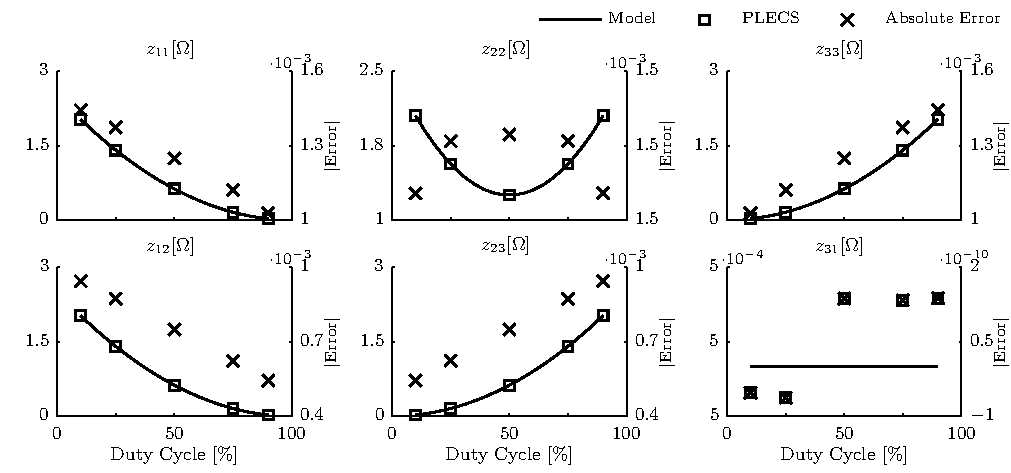
\includegraphics[page=1]{APEC_SIM_big}
  \centering
  \caption{SSL comparison between PLECS simulation and the proposed model.}
  \label{fig:sim_ssl}
\end{figure*}


\begin{figure*}[t]
  %\includegraphics[page=3]{APEC_SIM_big}
  \centering
  \caption{FSL comparison between PLECS simulation and the proposed model.}
  \label{fig:sim_fsl}
\end{figure*}

